\section*{Zadanie 33.}
\begin{task}
Narysować (w przekroju poprzecznym oraz pionowym i poziomym przekroju wzdłużnym) rozkłady pól 
$\textsl{E}$ i $\textsl{H}$ oraz prądów przewodzenia i przesunięcia dla fali bieżącej rodzaju $E_{01}$
w falowodzie kołowym. Jaki rodzaj w falowodzie prostokątnym  jest fizycznym odpowiednikiem tego rodzaju?\\
\end{task}

\begin{solution}

\begin{center}
$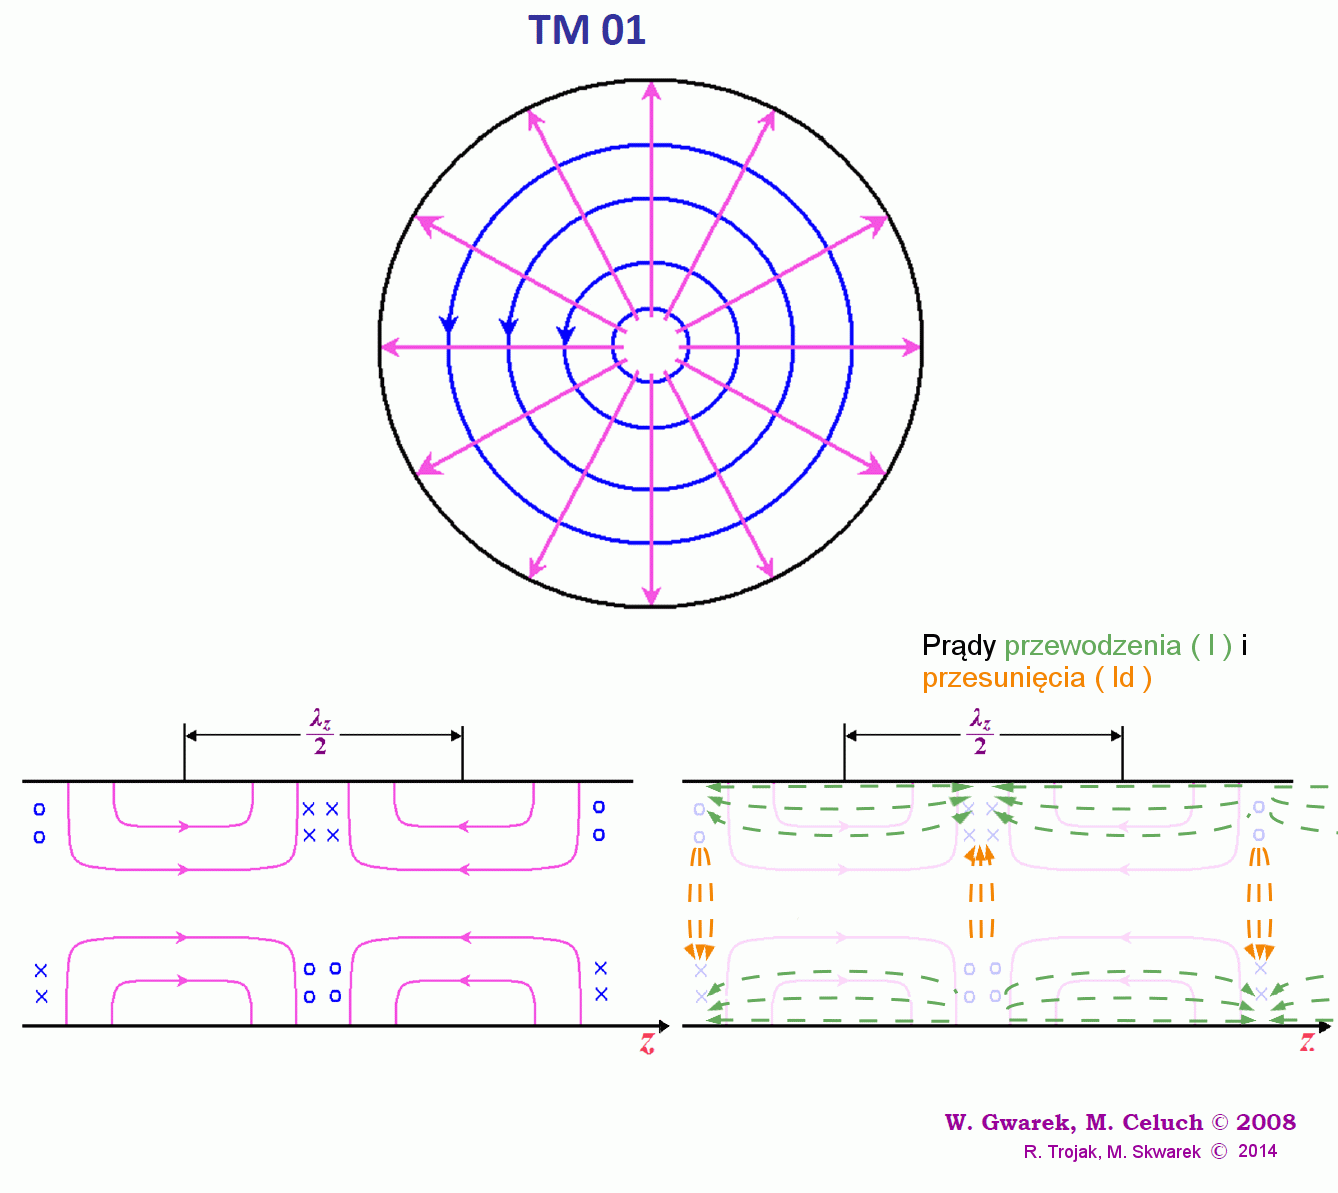
\includegraphics[scale=0.4]{33_1}$\\
\end{center}
Odpowiednikiem tego rodzaju w falowodzie prostokątnym jest rodzaj $E_{11}$\\
\end{solution}
